\chapter{Pianificazione}\label{chap:pianificazione}
La pianificazione è una parte fondamentale per ogni progetto. Essa ha il compito di definire le attività utili al completamento del progetto, pianificando il suo svolgimento tramite l'assegnazione intelligente di risorse ad ogni attività individuata, permettendo di valutare il reale grado di avanzamento dei lavori stimando e controllando i costi e le tempistiche effettive rispetto a quelle preventivate. Il prodotto di ogni periodo rappresenterà la \ccgloss{baseline} relativa agli obiettivi prefissati per quel lasso temporale.\\ \\
La pianificazione riportata di seguito tenta di raggiungere un buon grado di precisione non solo considerando l'analisi dei rischi individuati nella sezione precedente, ma anche tramite due particolari accorgimenti. La pianificazione generale avviene a ritroso, fissando il punto di arrivo previsto, con relativi vincoli finali, e individuando le attività che portano a tale obiettivo. La pianificazione dettagliata viene limitata ad un orizzonte temporale relativamente vicino, così che eventuali errori nella fase di pianificazione abbiano un impatto minore nello svolgimento del progetto, permettendo un'\ccgloss{agile} azione di riorganizzazione. 

\section{Modello adottato}
Dopo una prima discussione sui possibili \ccgloss{modelli di sviluppo} utilizzabili, nella realizzazione di questo progetto il gruppo ha deciso di adottare un modello di sviluppo agile, consigliato anche dall'azienda proponente.\\ \\
Il motivo di questa scelta è da ricercarsi principalmente nell'elevato grado di flessibilità che tale modello permette. Oltre a mettere in primo piano l'importanza dell'interazione continua e persistente con il proponente, importantissimo per l'analisi dei requisiti del prodotto finale, l'utilizzo di questo modello permette la verifica dello stato di avanzamento reale del progetto, mostrando al proponente quanto fatto, tramite la suddivisione del lavoro in incrementi a valore aggiuntivo.\\ \\
Per adottare questo modello di sviluppo, è stato deciso di utilizzare degli sprint dalla durata di due settimane l'uno, aiutandosi nella pianificazione e realizzazione del progetto utilizzando il \ccgloss{framework} \ccgloss{Scrum}, e accompagnando ogni consuntivo di periodo con una analisi retrospettiva.

\section{Requirements and Technology Baseline}
\label{pianificazione:rtb}

\subsection{Primo sprint: 2023/11/06 - 2023/11/19}
\subsubsection{Obiettivi}
\begin{itemize} 
    \item Inizio stesura delle Norme di Progetto;
    \item Stesura template dei documenti per il progetto;
    \item Inizio stesura del Piano di Progetto;
    \item Stesura iniziale di \ccgloss{Use cases};
    \item Impostare compilazione automatica documenti in LaTeX;
    \item Impostare il funzionamento dell'issue traking system \ccgloss{Jira}.
\end{itemize}

\begin{figure}[h!]
    \centering  
    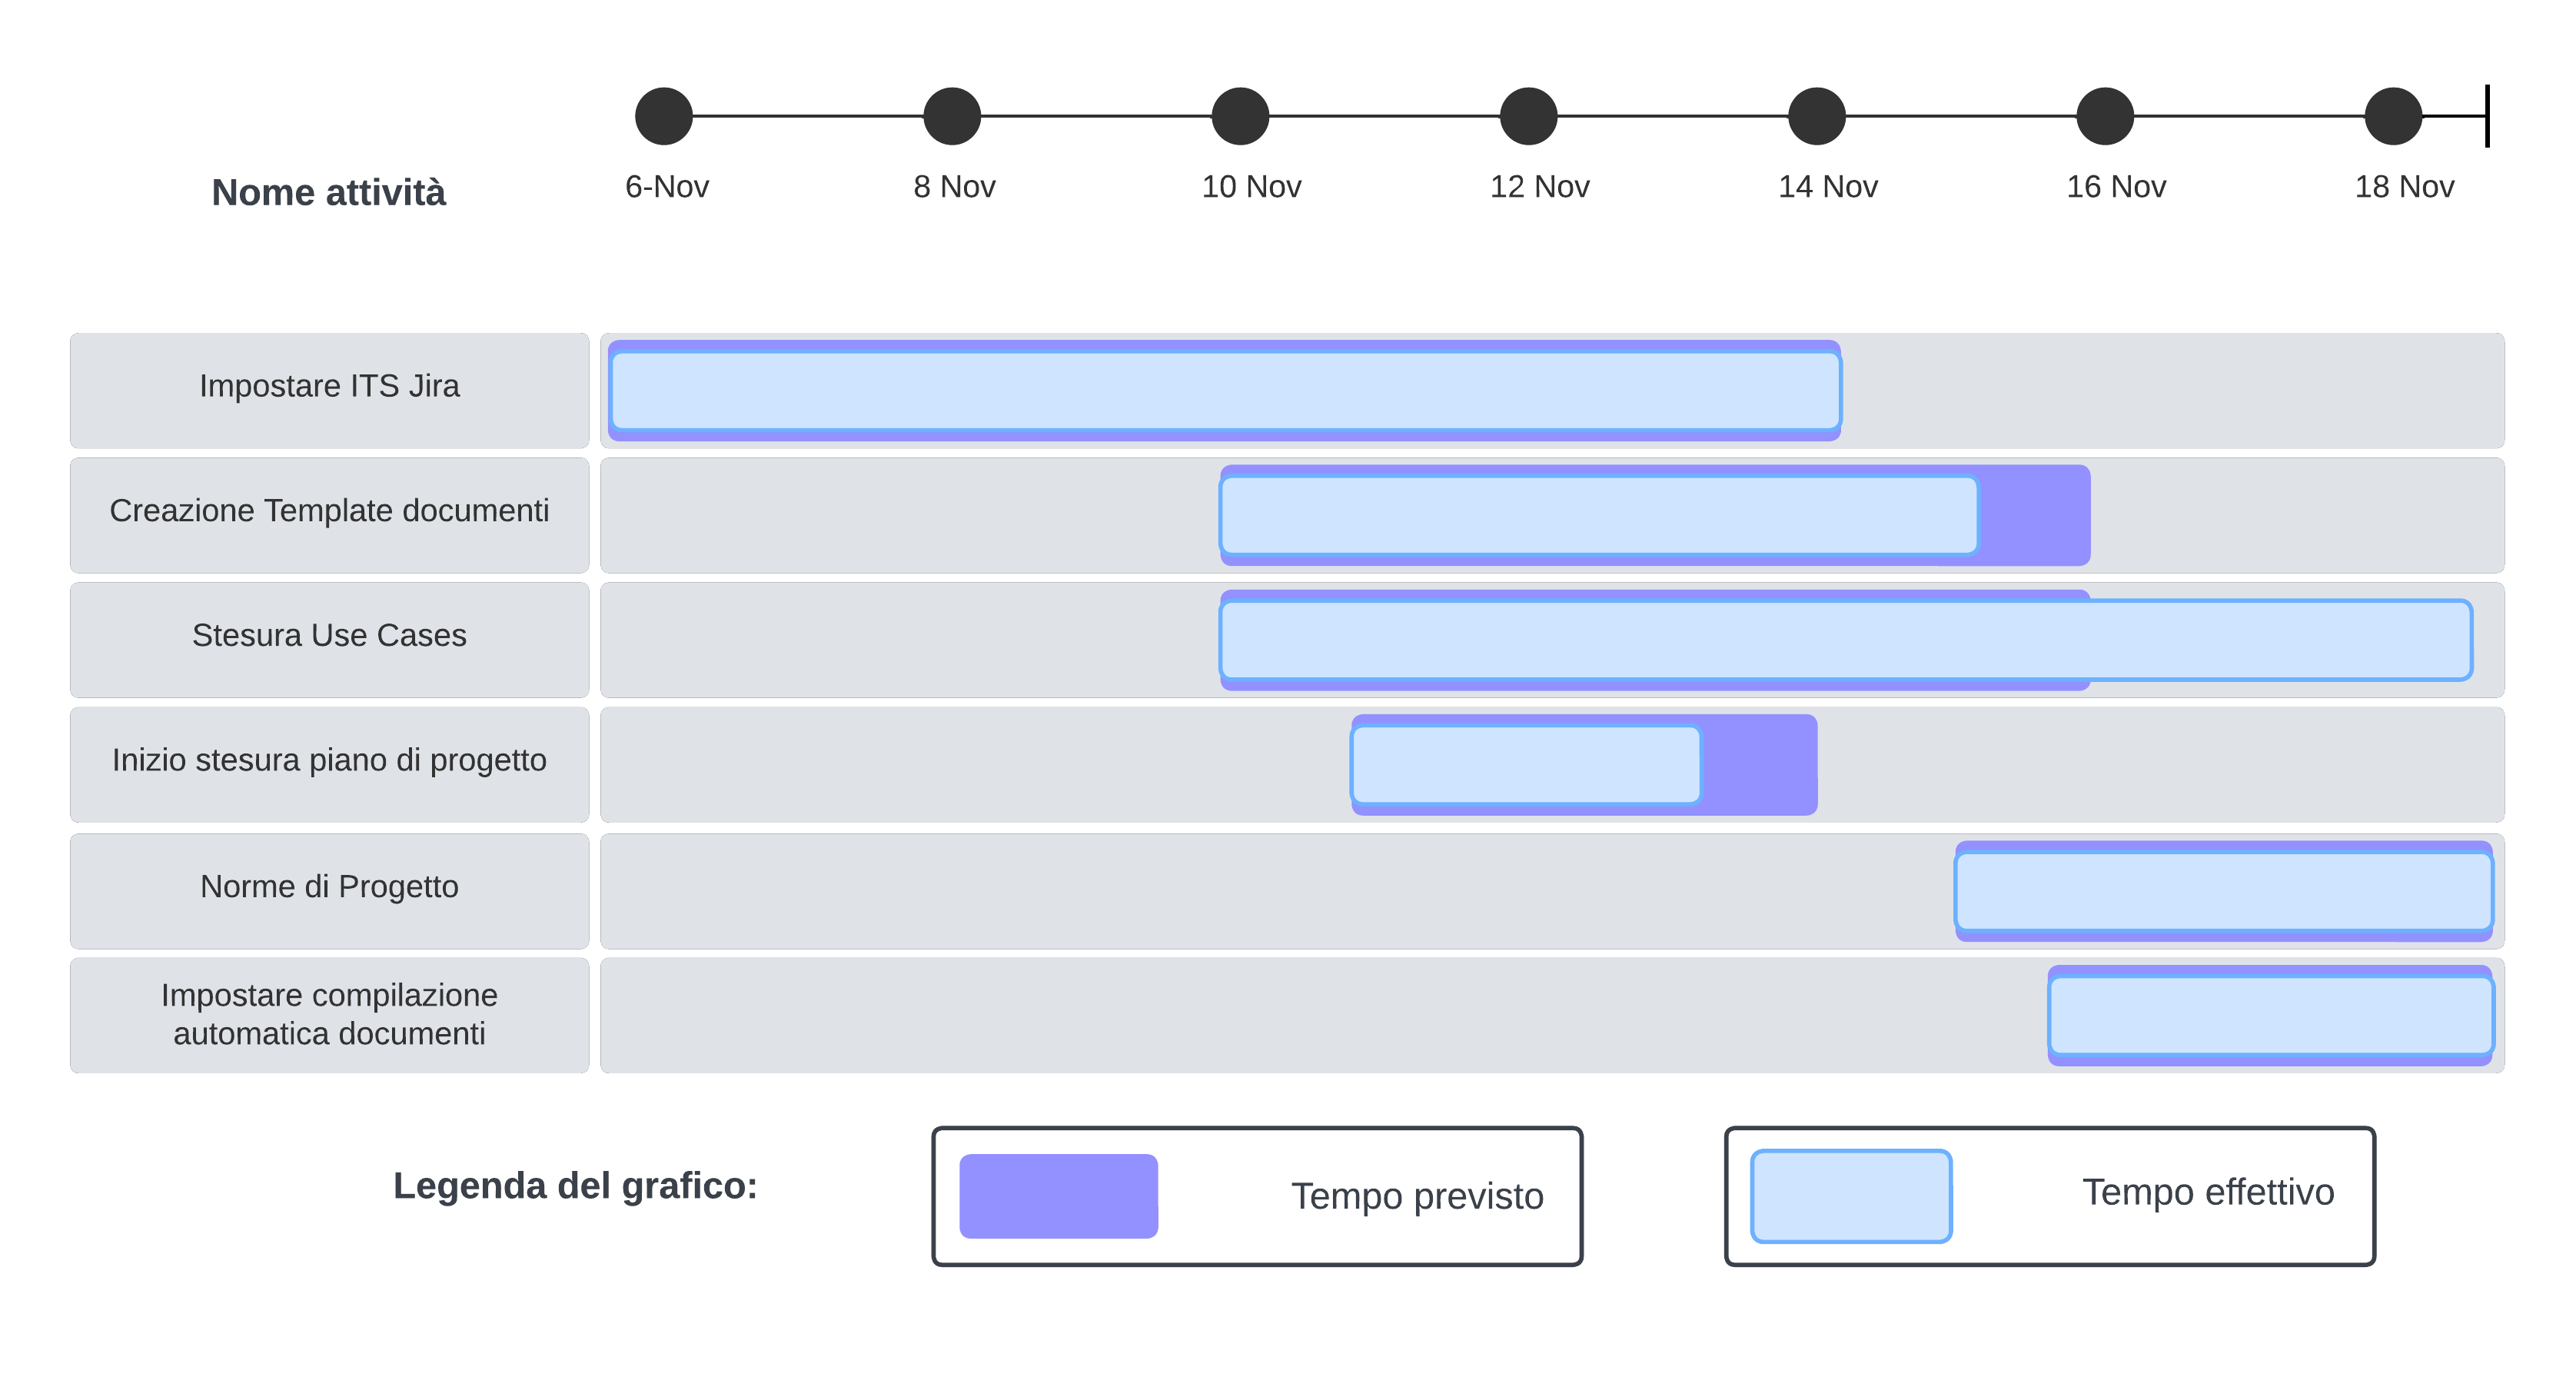
\includegraphics[width=\textwidth]{Roadmap1sprint.png}
    \caption{\ccgloss{Diagramma di \ccgloss{Gantt}} del primo sprint}
    \label{fig:roadmap1s}
\end{figure}
\newpage

\subsection{Secondo sprint: 2023/11/20 - 2023/12/03}
\subsubsection{Obiettivi}
\begin{itemize}
    \item Proseguire la stesura del Piano di Progetto;
    \item Perfezionare il documento di Analisi dei requisiti;
    \item Ampliamento delle Norme di Progetto;
    \item Ultimazione stesura del Glossario;
    \item Stesura del Piano di Qualifica;
    \item Progettazione del \ccgloss{PoC};
    \item Programmazione del PoC;
    \item \ccgloss{Bug} Fix della compilazione automatica dei documenti \LaTeX.
\end{itemize}

\begin{figure}[h!]
    \centering  
    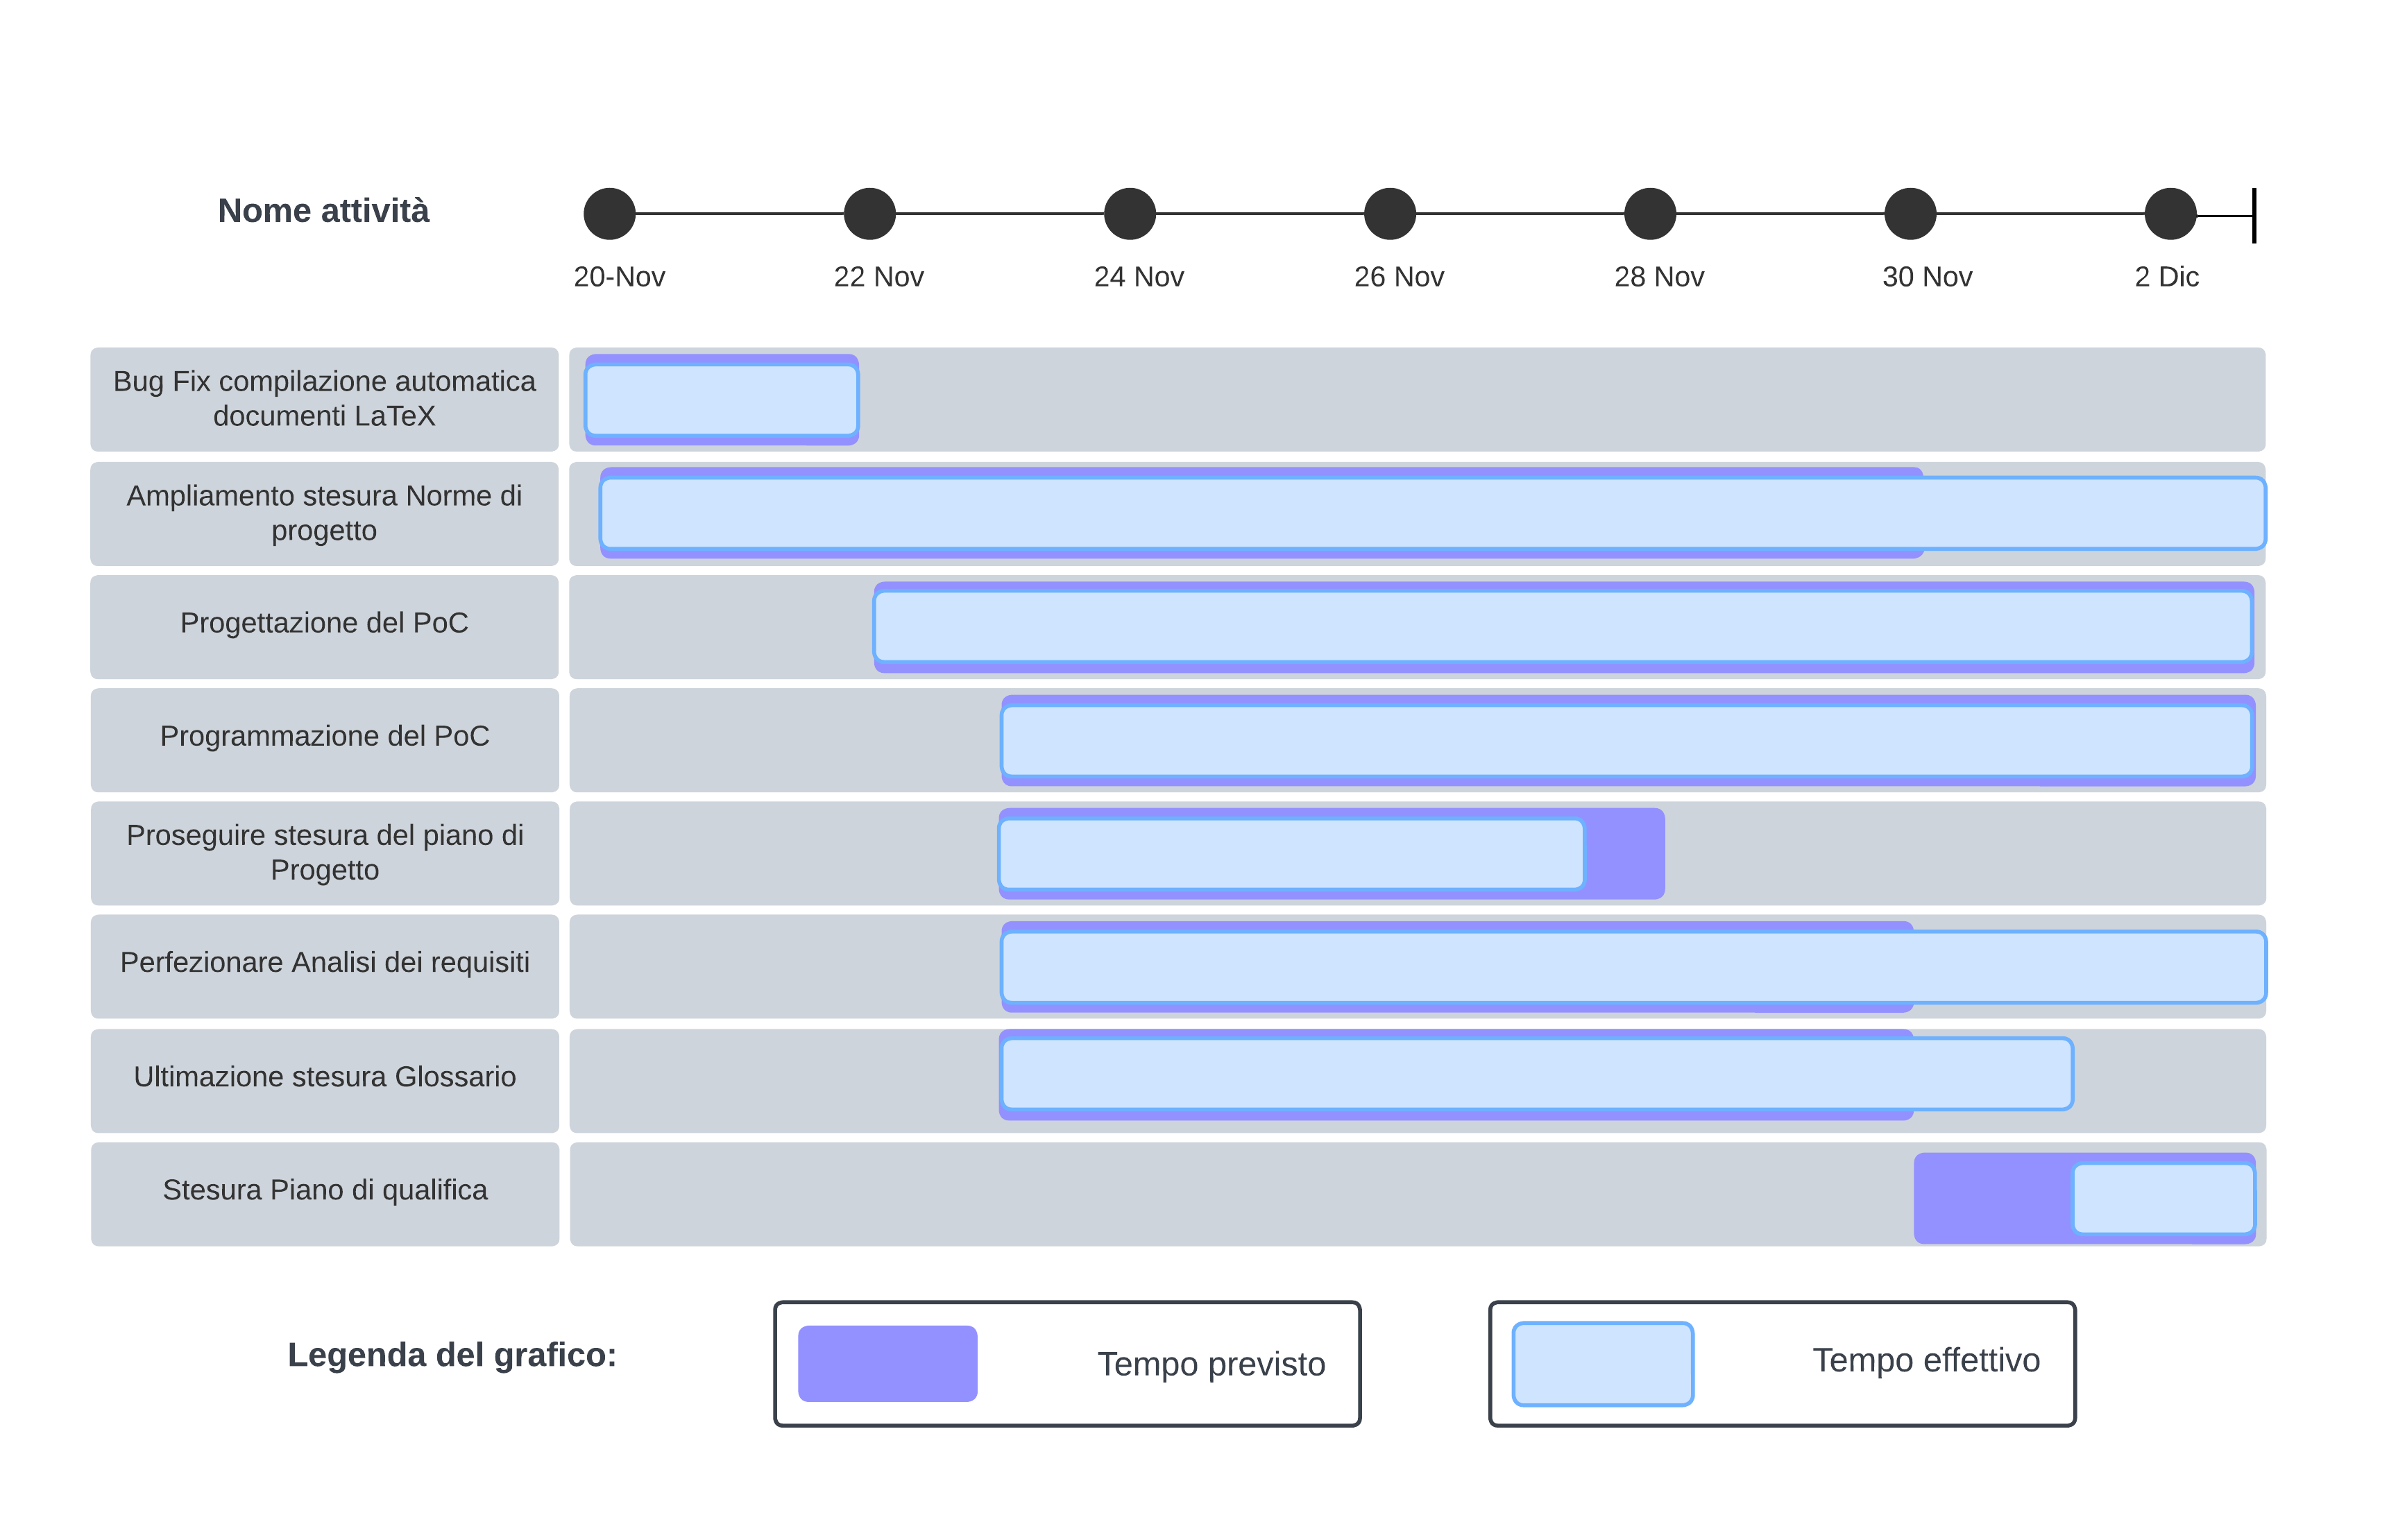
\includegraphics[width=\textwidth]{Roadmap2sprint.png}
    \caption{Diagramma di Gantt del secondo sprint}
    \label{fig:roadmap2s}
\end{figure}
\newpage

\subsection{Terzo sprint: 2023/12/04 - 2023/12/17}
\subsubsection{Obiettivi}
\begin{itemize}
    \item Aggiornamento del Piano di Progetto;
    \item Conclusione stesura delle Norme di Progetto;
    \item Conclusione stesura del Piano di Qualifica;
    \item Conclusione stesura dell'Analisi dei Requisiti;
    \item Conclusione progettazione PoC;
    \item Conclusione programmazione PoC.
\end{itemize}


\begin{figure}[h!]
    \centering  
    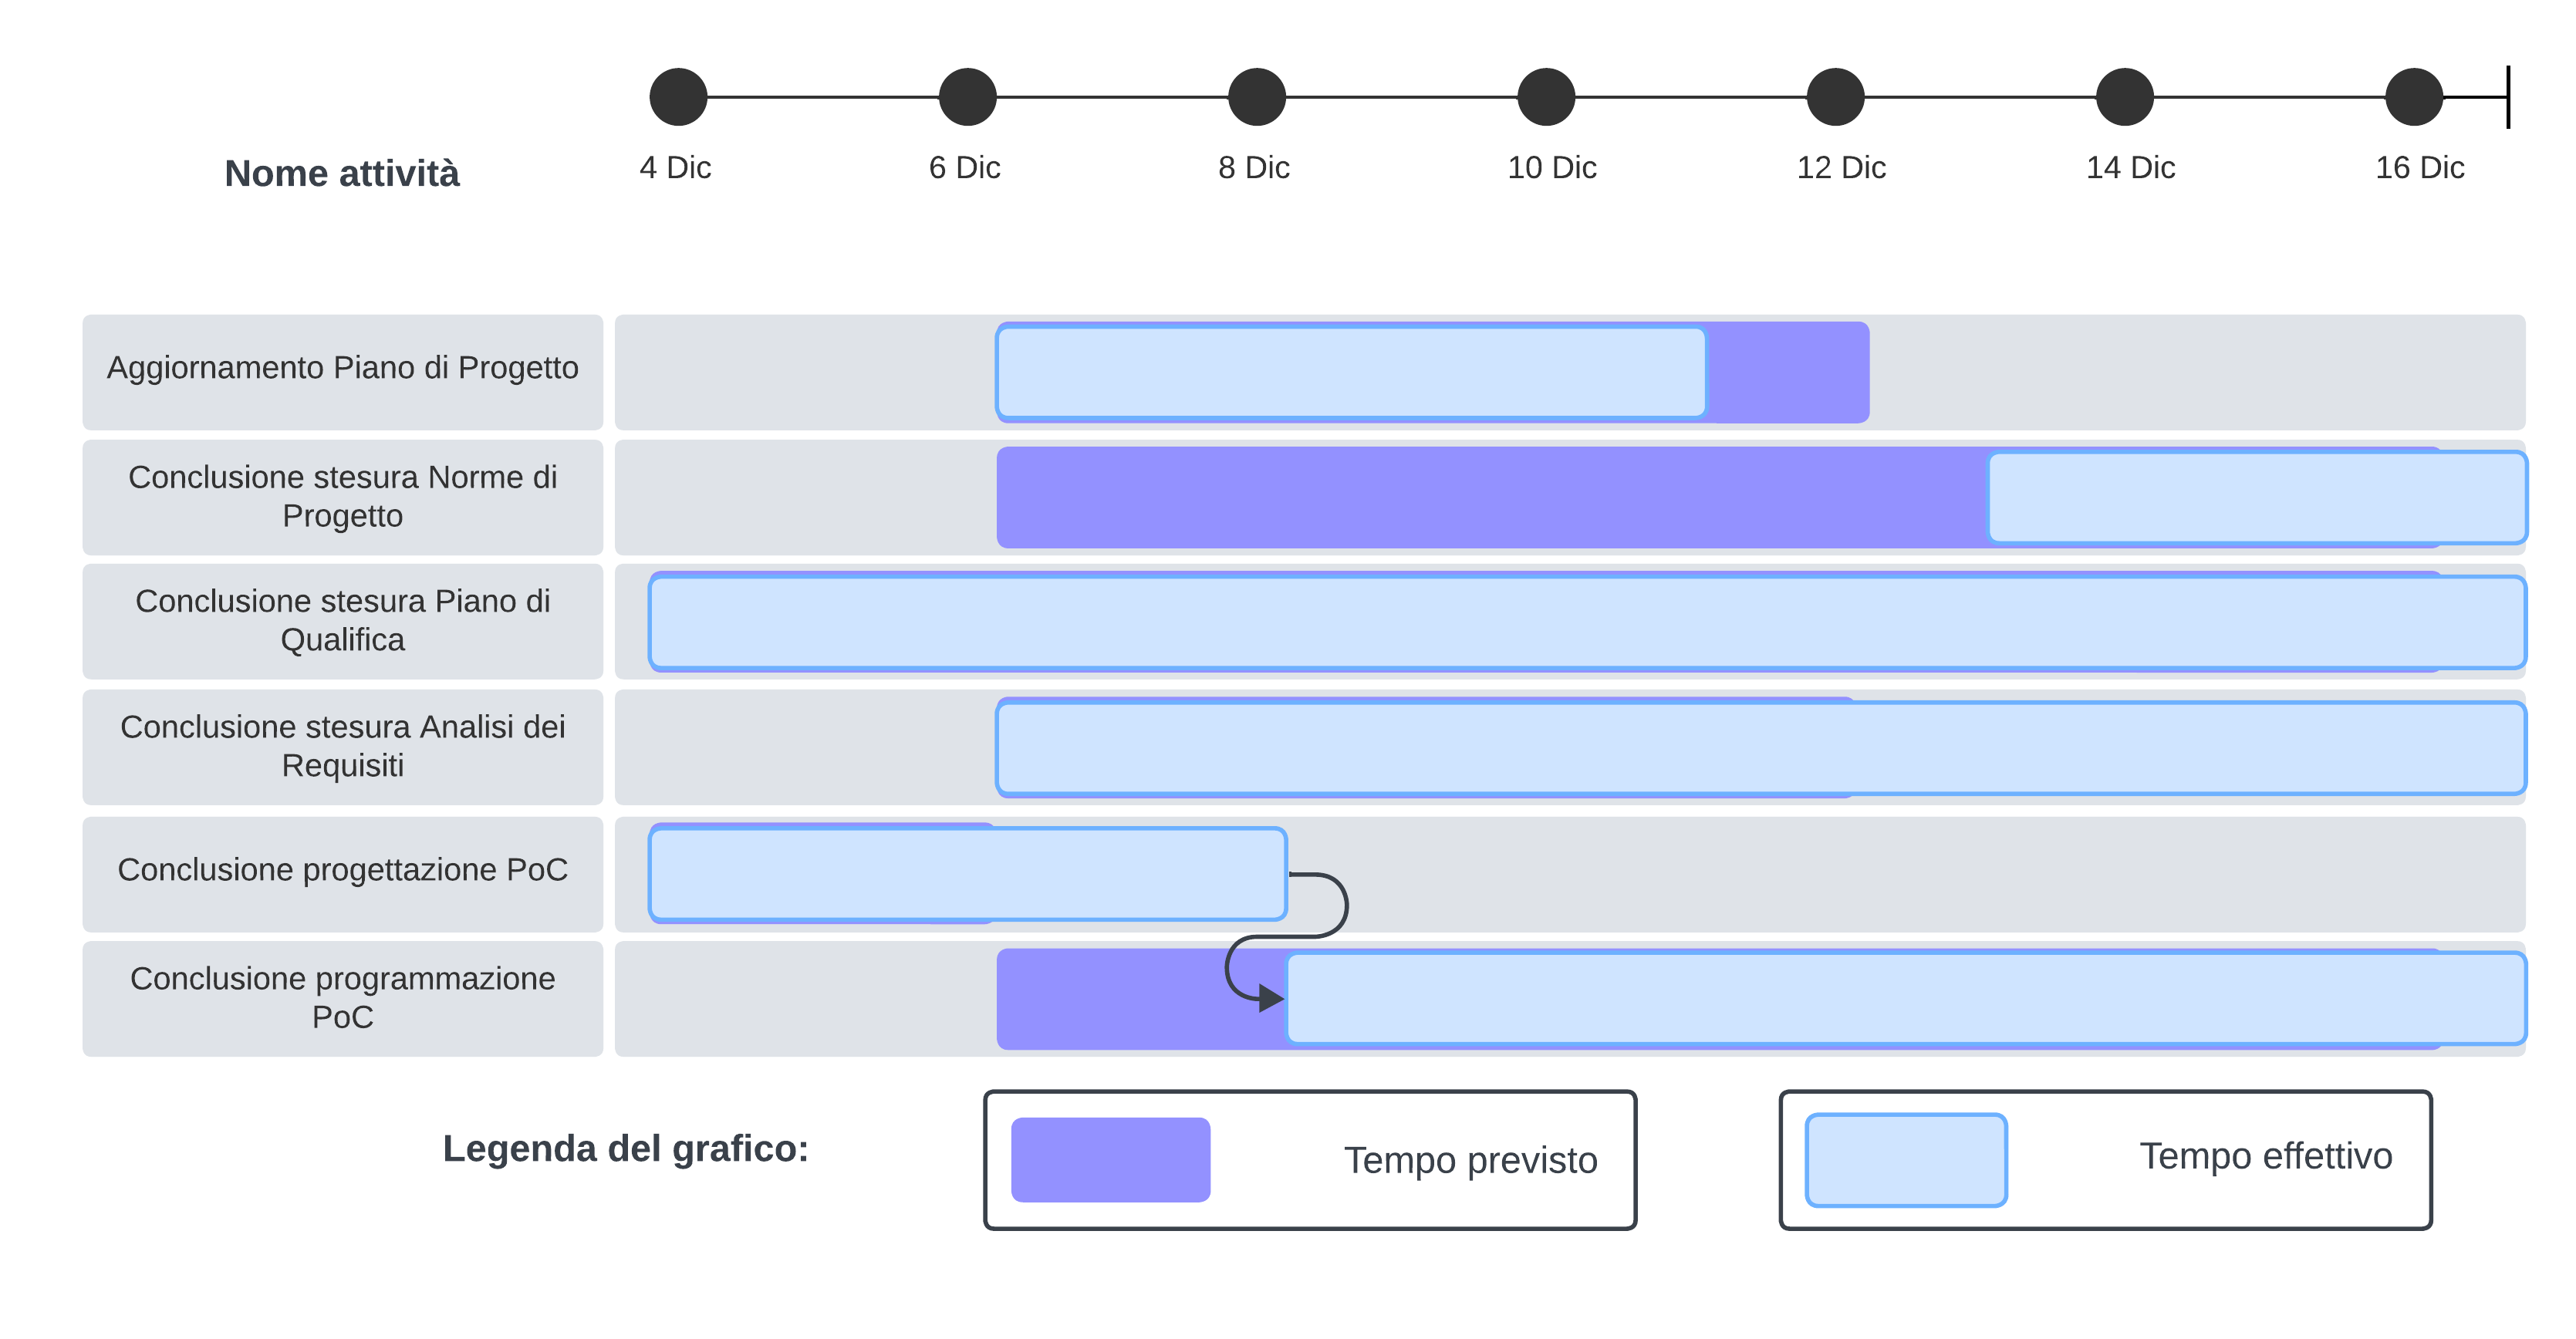
\includegraphics[width=\textwidth]{Roadmap3sprint.png}
    \caption{Diagramma di Gantt del terzo sprint}
    \label{fig:roadmap3s}
\end{figure}
\newpage

\subsection{Quarto sprint: 2023/12/18 - 2023/12/31}
\subsubsection{Obiettivi}
\begin{itemize}
    \item Inserimento di nuovi termini nel Glossario;
    \item Concludere il documento di Analisi dei requisiti;
    \item Conclusione delle Norme di Progetto;
    \item Conclusione del Piano di Qualifica;
    \item Aggiornamento del Piano di Progetto;
    \item Conclusione PoC.
\end{itemize}

\begin{figure}[h!]
    \centering  
    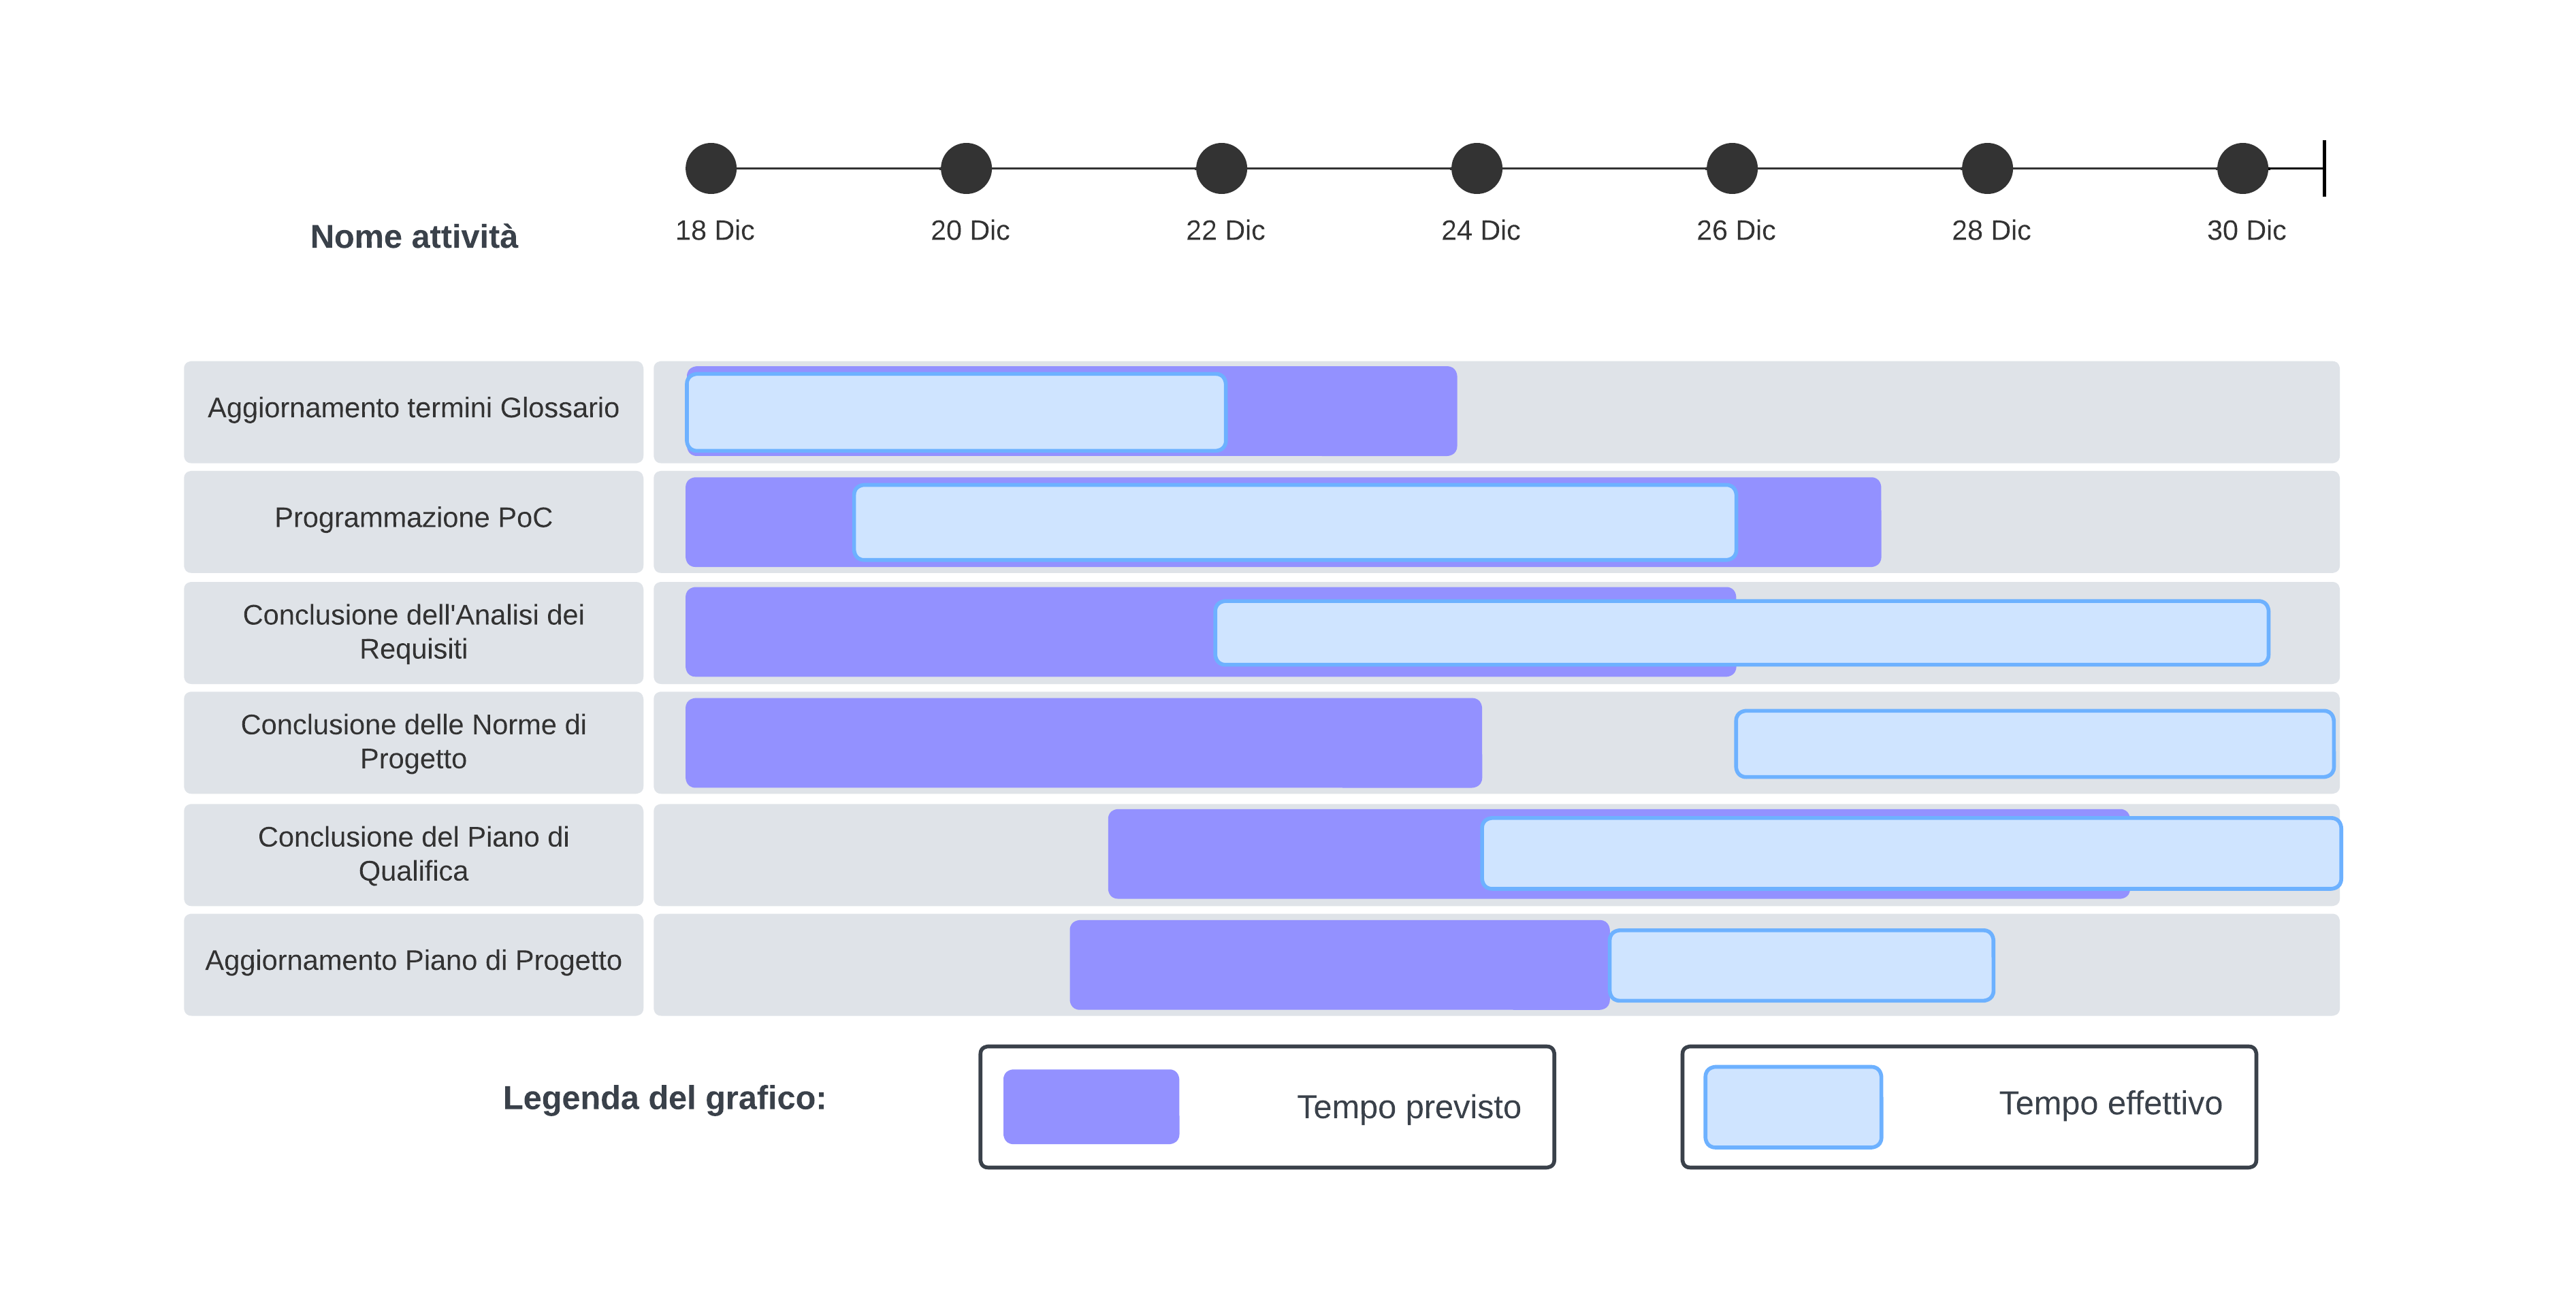
\includegraphics[width=\textwidth]{Roadmap4sprint.png}
    \caption{Diagramma di Gantt del quarto sprint}
    \label{fig:roadmap4s}
\end{figure}
\newpage

\subsection{Quinto sprint: 2024/01/01 - 2024/01/14}
\subsubsection{Obiettivi}
\begin{itemize}
    \item Conclusione del Glossario;
    \item Conclusione delle Norme di Progetto;
    \item Aggiornamento del Piano di Qualifica;
    \item Aggiornamento del Piano di Progetto;
    \item Aggiornamento e conclusione PoC;
    \item Preparazione del materiale per revisione \ccgloss{RTB}.
\end{itemize}

\begin{figure}[h!]
    \centering  
    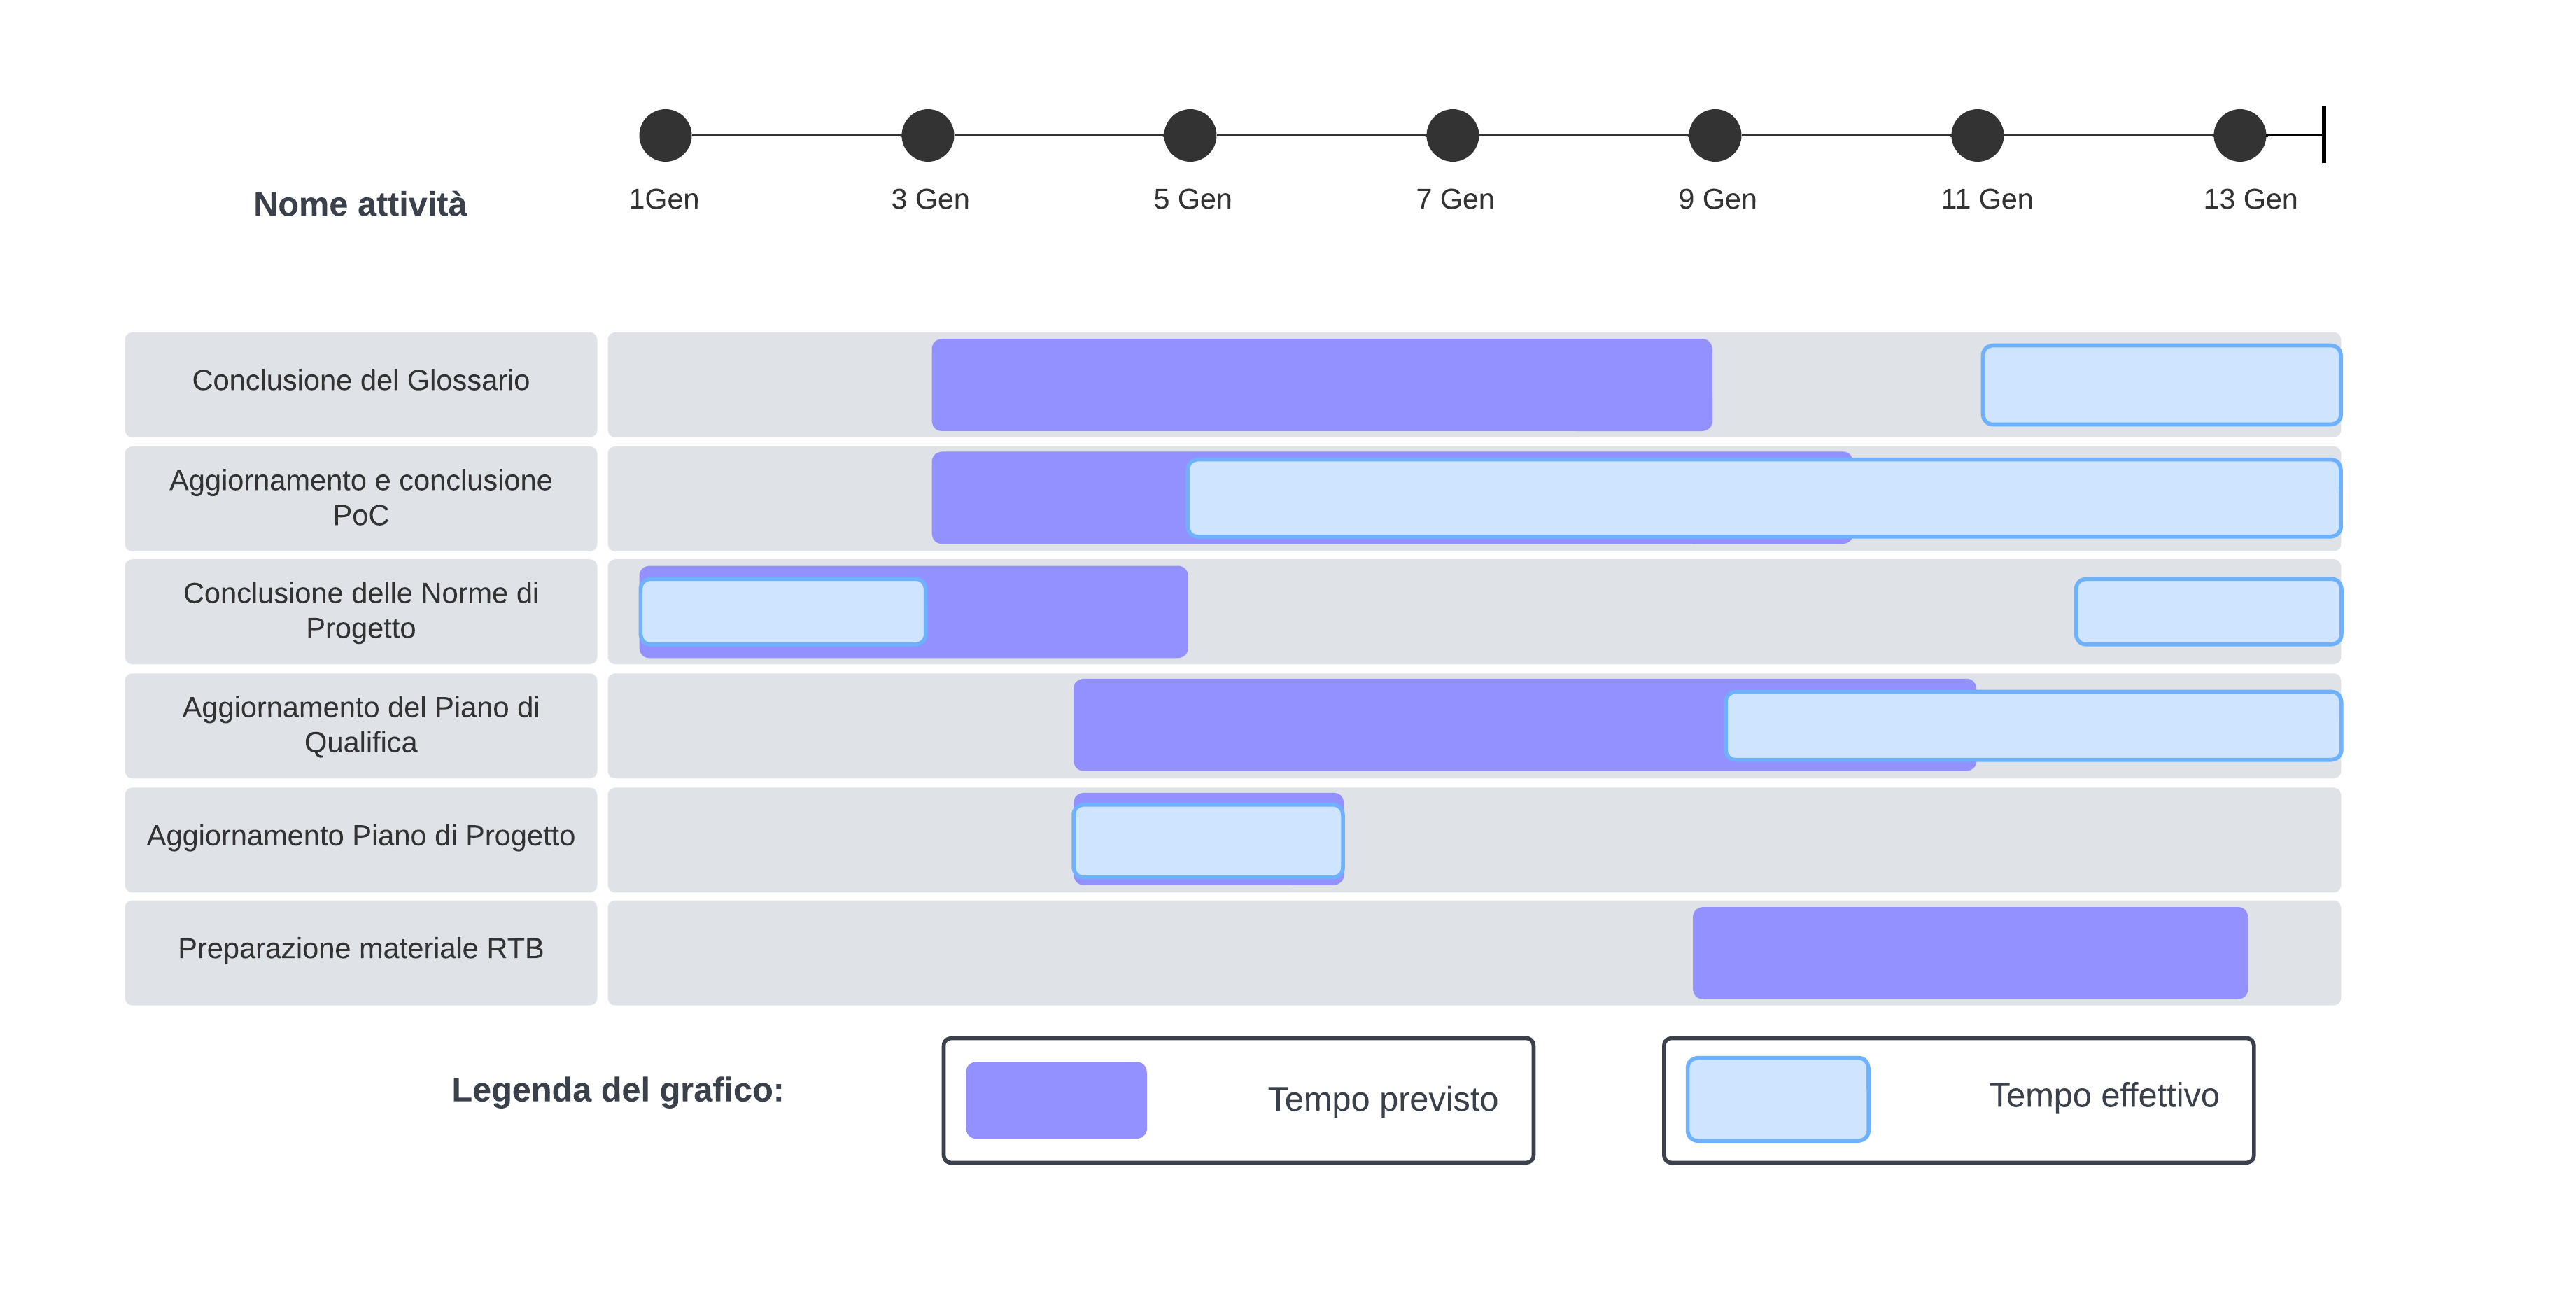
\includegraphics[width=\textwidth]{Roadmap5sprint.png}
    \caption{Diagramma di Gantt del quinto sprint}
    \label{fig:roadmap5s}
\end{figure}
\newpage

\subsection{Sesto sprint: 2024/01/15 - 2024/01/28}
\subsubsection{Obiettivi}
\begin{itemize}
    \item Aggiornamento e conclusione dell'Analisi dei requisiti;
    \item Aggiornamento del Piano di Progetto;
    \item Conclusione delle Norme di Progetto;
    \item Aggiornamento del Glossario;
    \item Aggiornamento e conclusione PoC;
    \item Preparazione del materiale per revisione RTB;
    \item Invio richiesta per revisione RTB;
    \item Inizio pianificazione e progettazione in ottica \ccgloss{MVP}.
\end{itemize}

\begin{figure}[h!]
    \centering  
    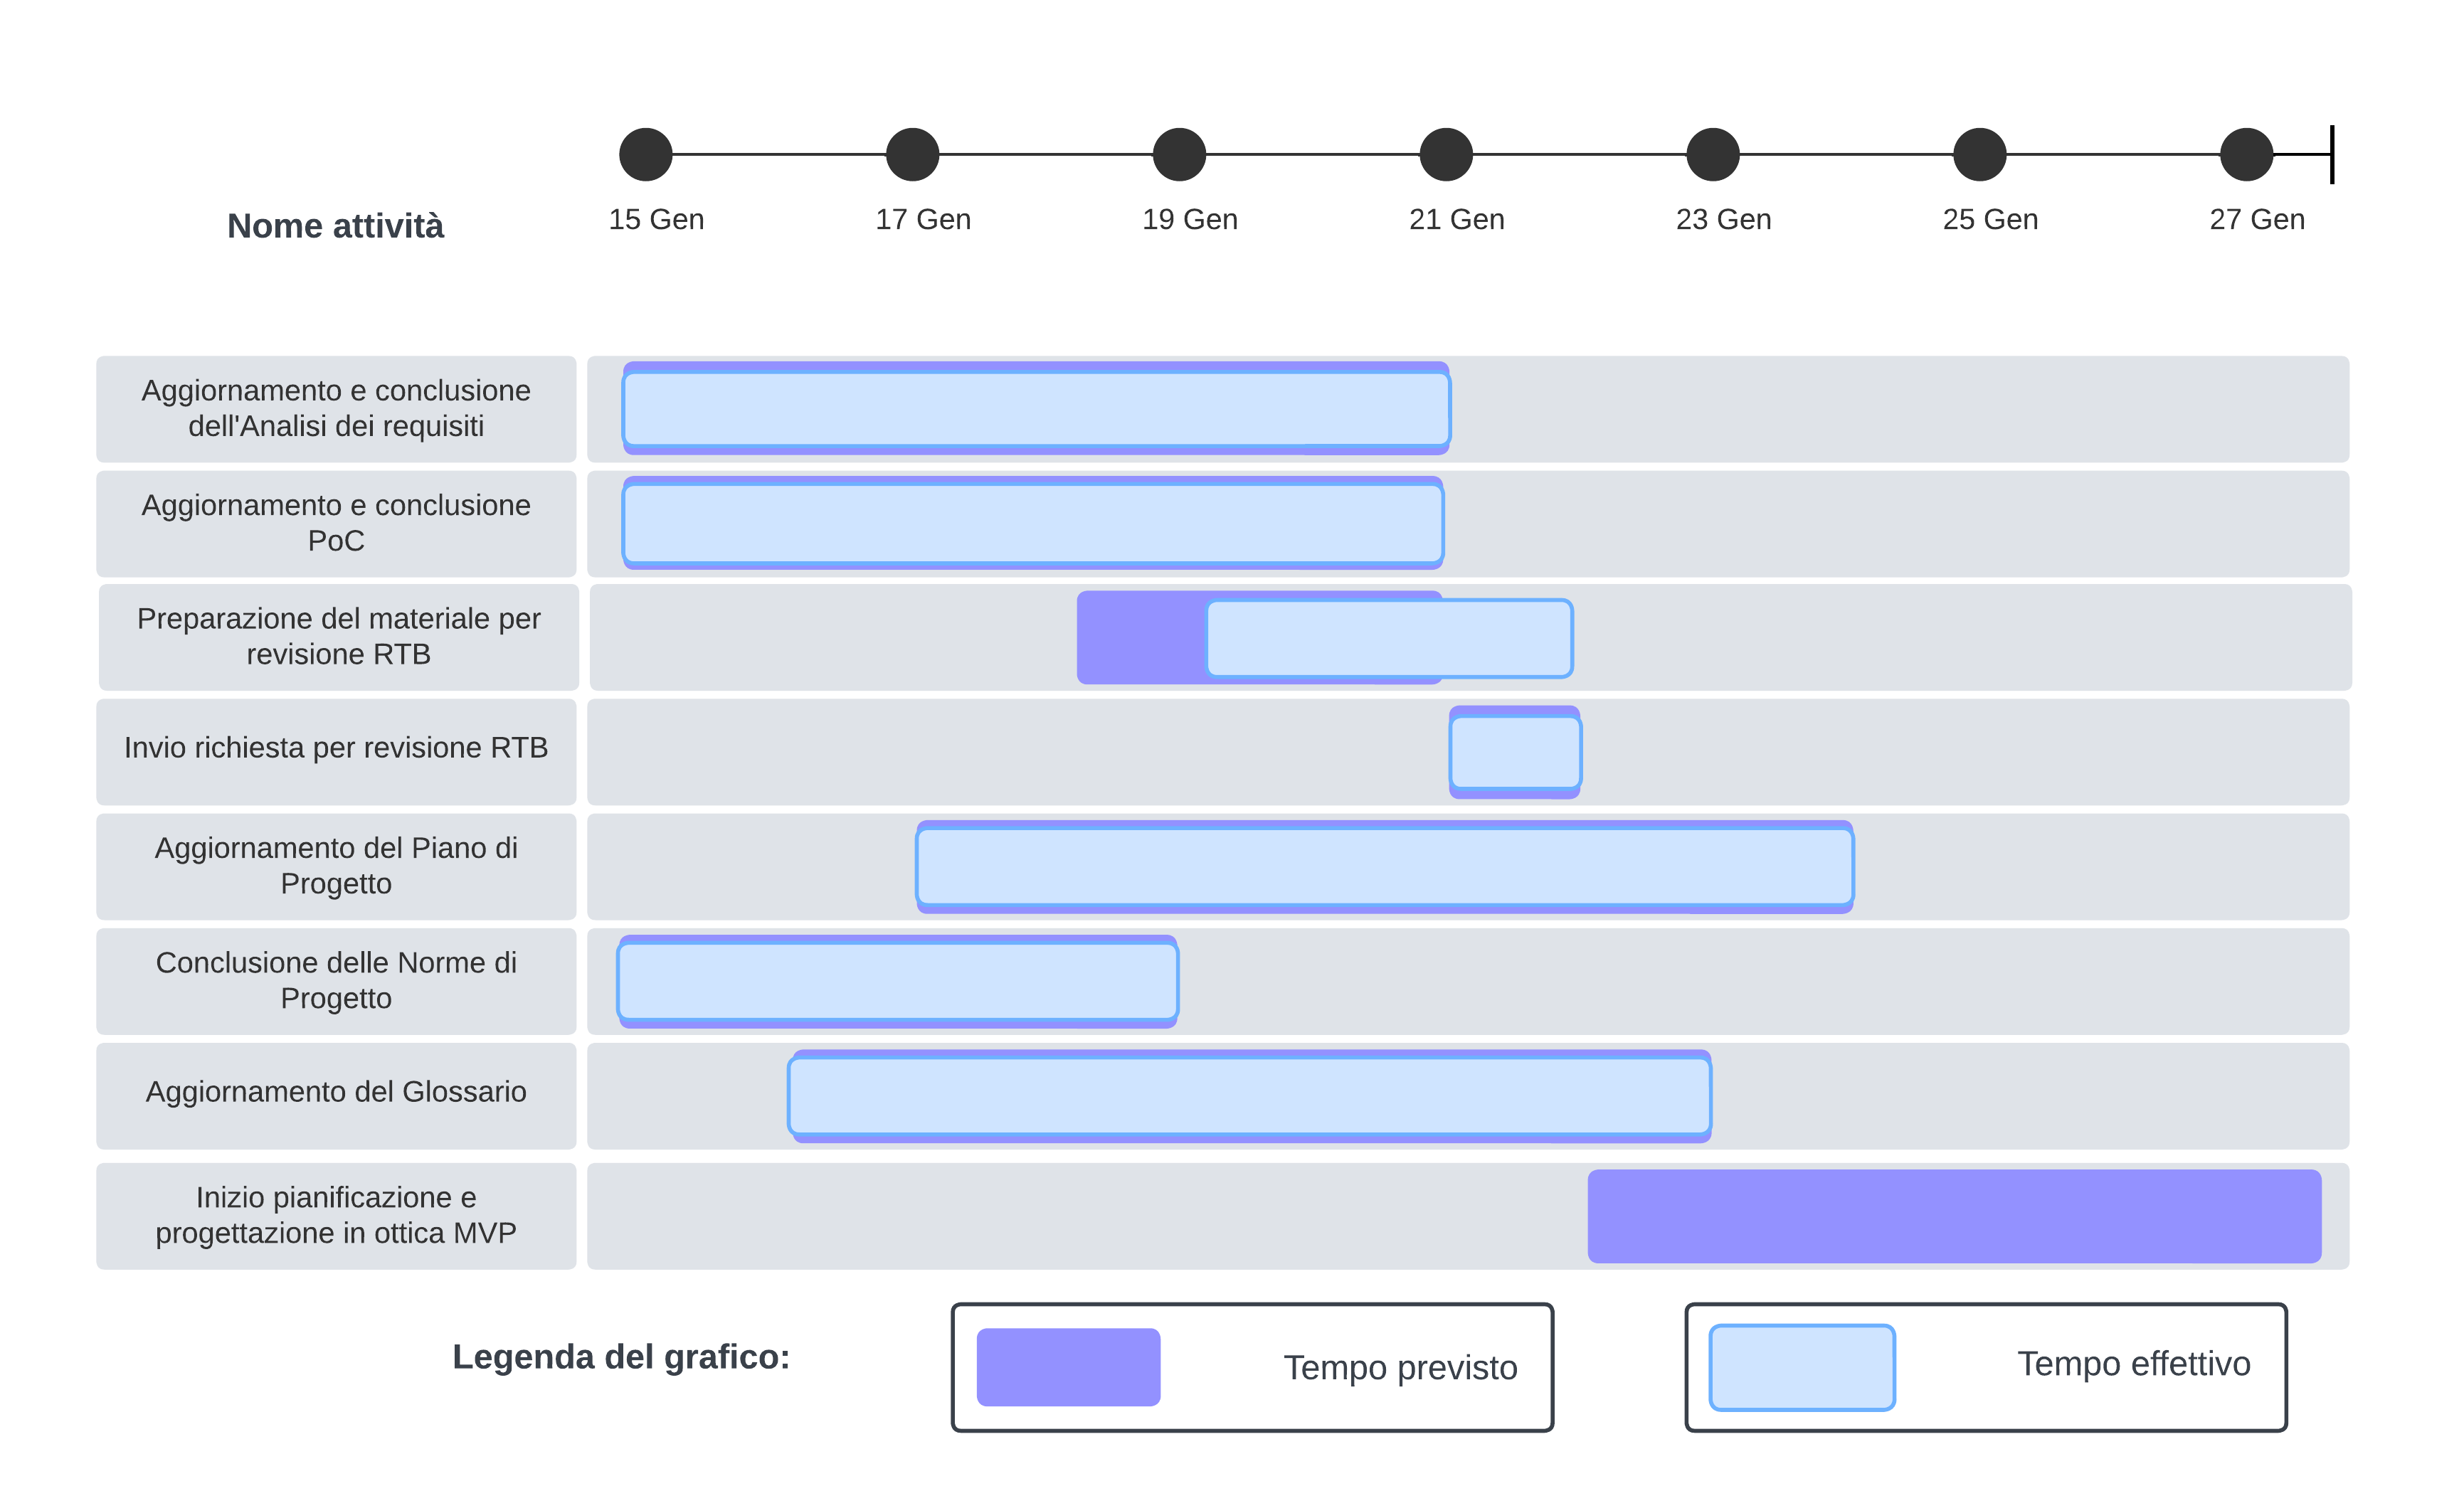
\includegraphics[width=\textwidth]{Roadmap6sprint.png}
    \caption{Diagramma di Gantt del sesto sprint}
    \label{fig:roadmap6s}
\end{figure}
\newpage

\subsection{Settimo sprint: 2024/01/29 - 2024/02/11}
\subsubsection{Obiettivi}
\begin{itemize}
    \item Correzioni all'Analisi dei Requisiti;
    \item Conclusione Piano di Qualifica;
    \item Conclusione Glossario;
    \item Aggiornamento Piano di Progetto;
    \item Invio domanda per la seconda parte della revisione RTB;
    \item Preparazione per la seconda parte della revisione RTB;
    \item Inizio pianificazione e progettazione in ottica MVP.
\end{itemize}

\begin{figure}[h!]
    \centering  
    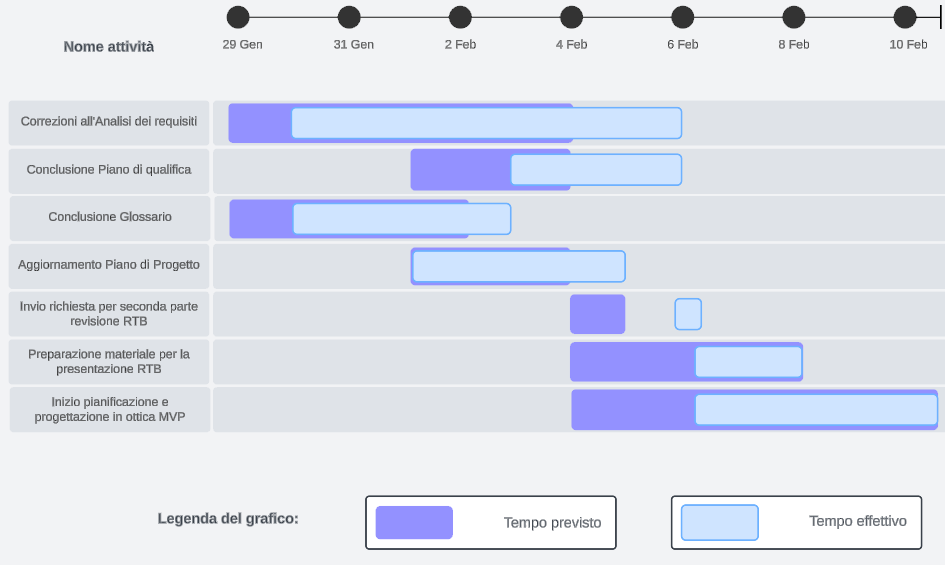
\includegraphics[width=\textwidth]{Roadmap7sprint.png}
    \caption{Diagramma di Gantt del settimo sprint}
    \label{fig:roadmap7s}
\end{figure}
\newpage

\section{Product Baseline}
Dopo l'analisi dei costi intrapresi durante la RTB e dei relativi tempi di completamento, viene confermata come data di conclusione del progetto il \textit{2024/04/08}.\\Sulla base di quanto discusso nella riunione descritta dal Verbale\_2024\_02\_05\_v1.0 viene deciso di risuddividere le ore rimanenti per ogni \ccgloss{ruolo} restando comunque nel budget previsto all'inizio del progetto, ovvero \textit{12.985€}.\\Tale risuddivisione è visibile alla sezione \ref{sec:risuddivisione} di questo documento.
\newpage

\subsection{Ottavo sprint: 2024/02/12 - 2024/02/25}
\subsubsection{Obiettivi}
\begin{itemize}
    \item Correzioni all'Analisi dei Requisiti post RTB;
    \item Correzioni e aggiornamento Piano di Qualifica;
    \item Correzioni e aggiornamento Norme di Progetto;
    \item Aggiornamento Glossario;
    \item Aggiornamento Piano di Progetto;
    \item Aggiornamento Specifica Architetturale;
    \item Progettazione MVP;
    \item Inizio programmazione.
\end{itemize}

\begin{figure}[h!]
    \centering  
    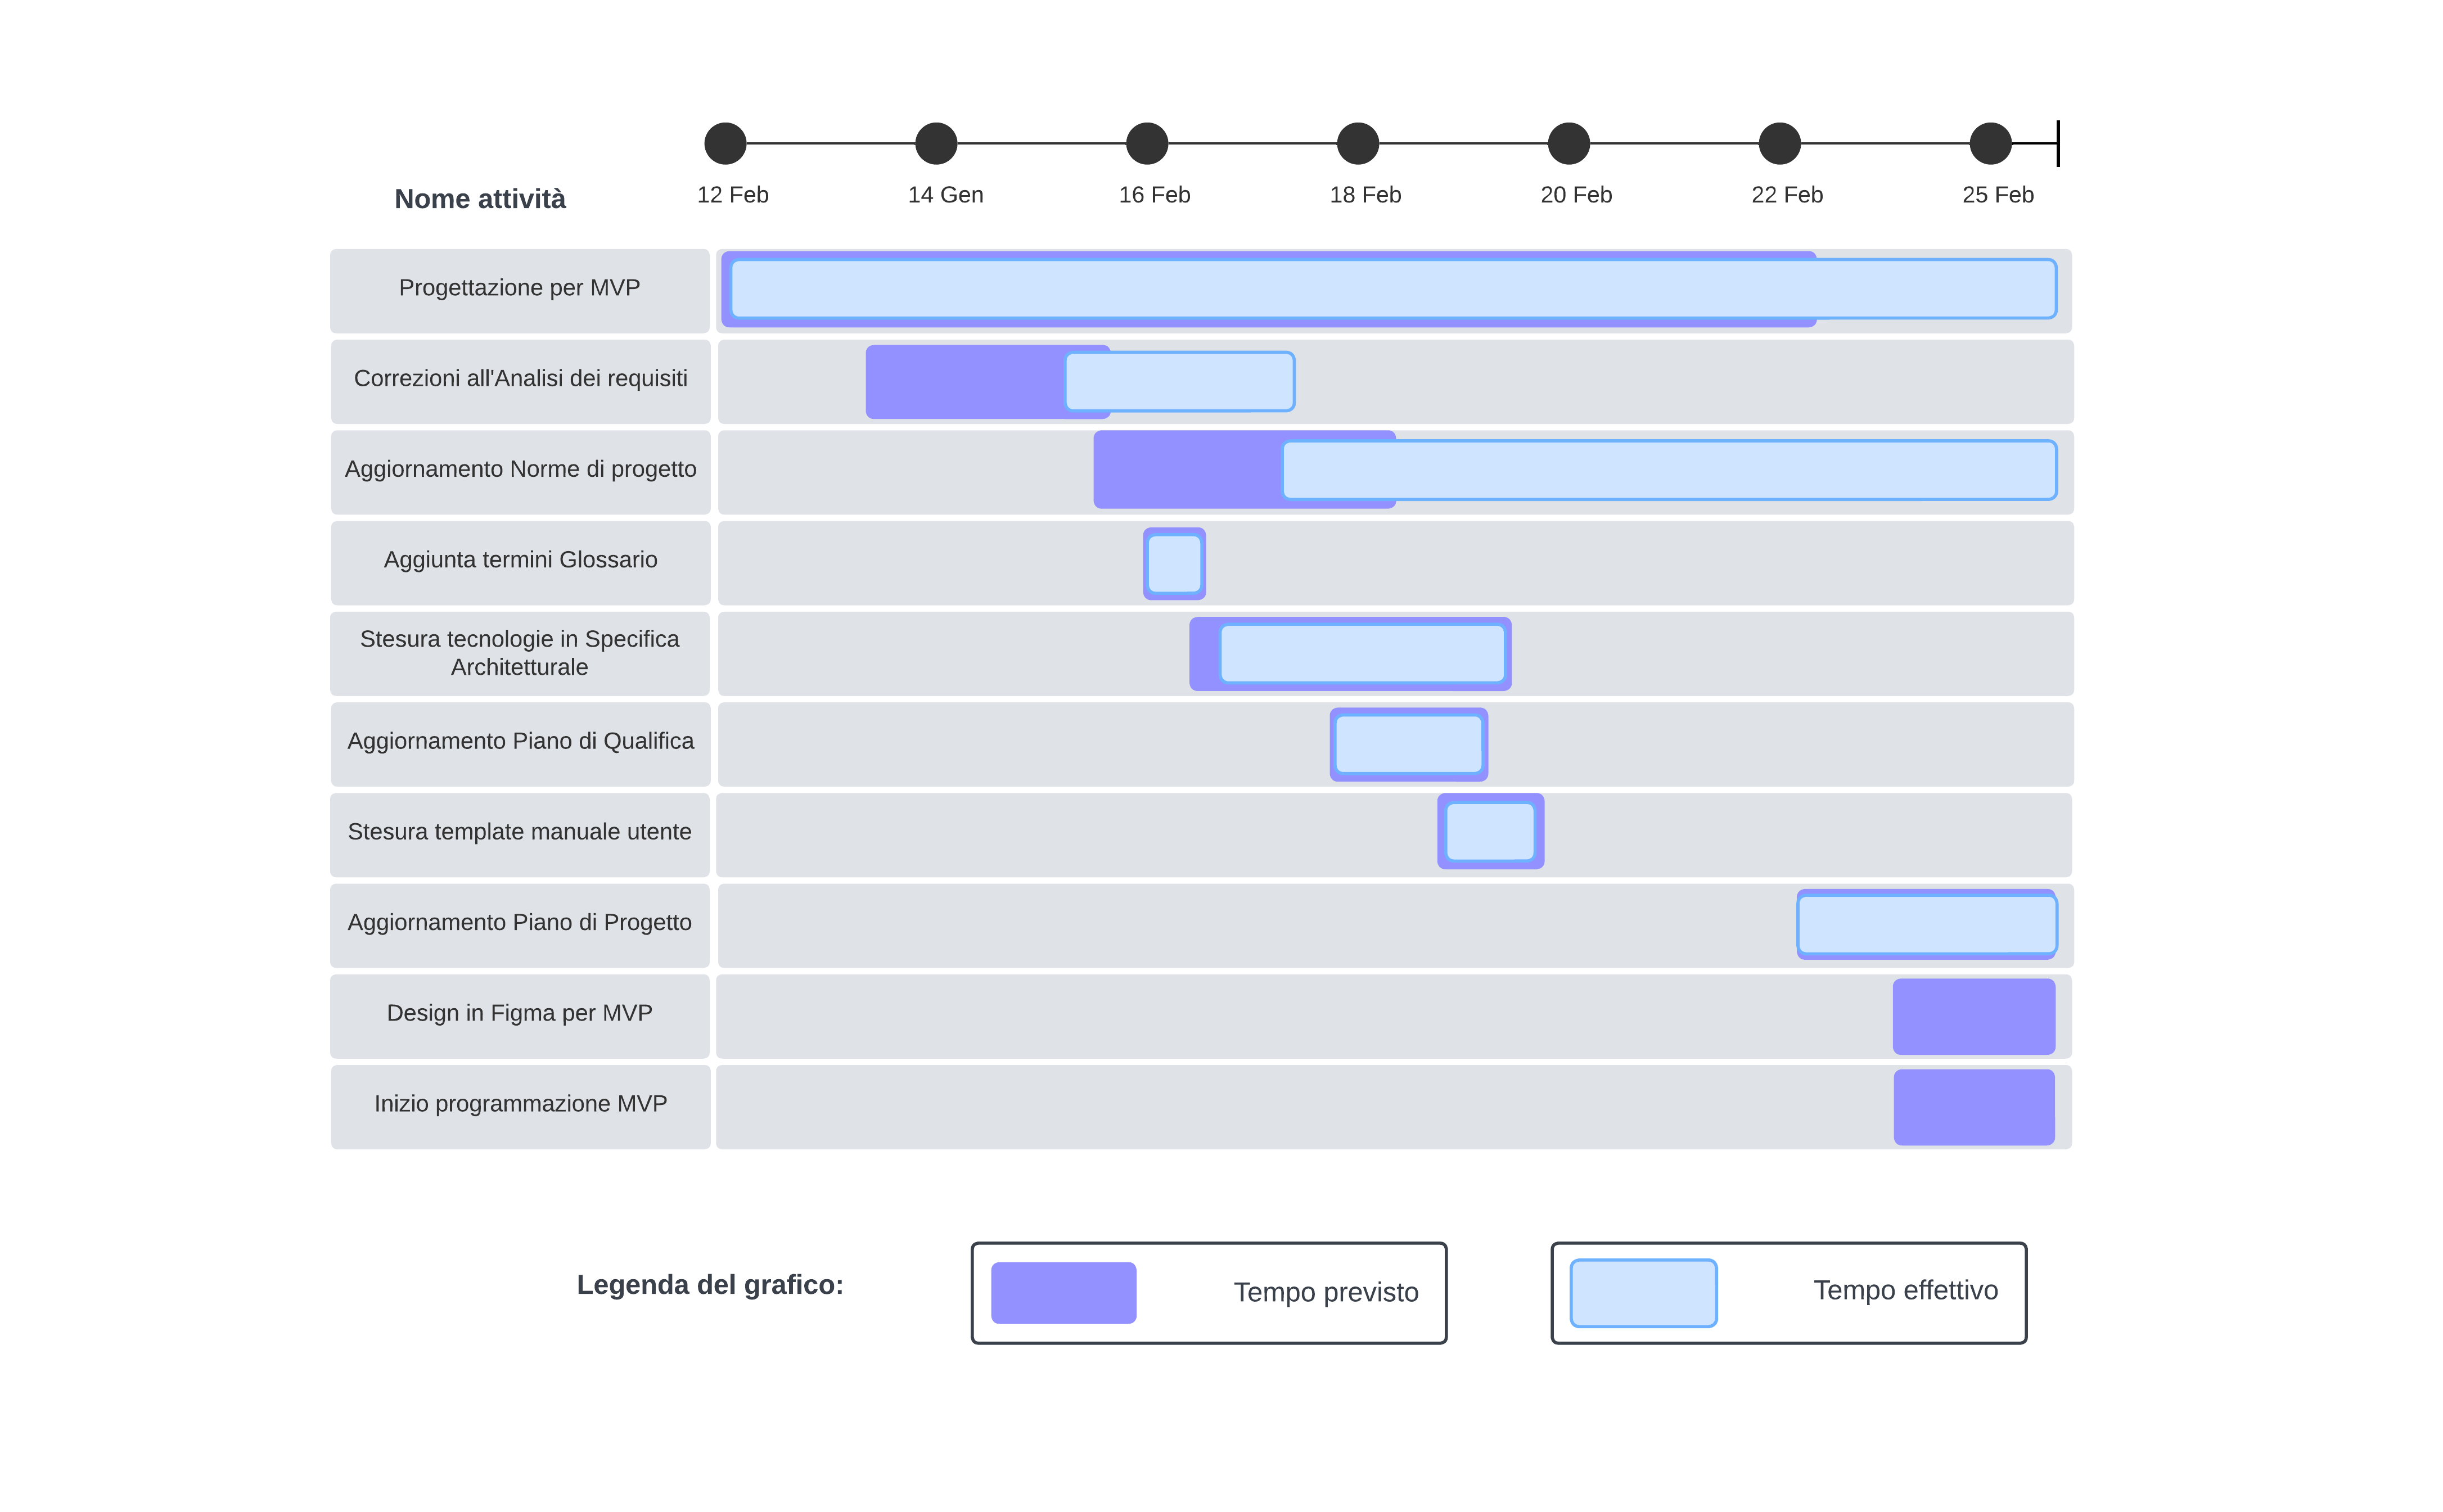
\includegraphics[width=\textwidth]{Roadmap8sprint.png}
    \caption{Diagramma di Gantt dell'ottavo sprint}
    \label{fig:roadmap8s}
\end{figure}
\newpage

\subsection{Nono sprint: 2024/02/26 - 2024/03/10}
\subsubsection{Obiettivi}
\begin{itemize}
    \item Aggiornamento Piano di Qualifica;
    \item Aggiornamento Specifica Architetturale;
    \item Aggiornamento Piano di Progetto;
    \item Progettazione e codifica aggiunta documenti;
    \item Progettazione e codifica eliminazione documenti;
    \item Progettazione e codifica ricerca documenti;
    \item Progettazione e codifica domanda risposta chatbot;
    \item Progettazione e codifica fonti risposta.
\end{itemize}

\begin{figure}[h!]
    \centering
    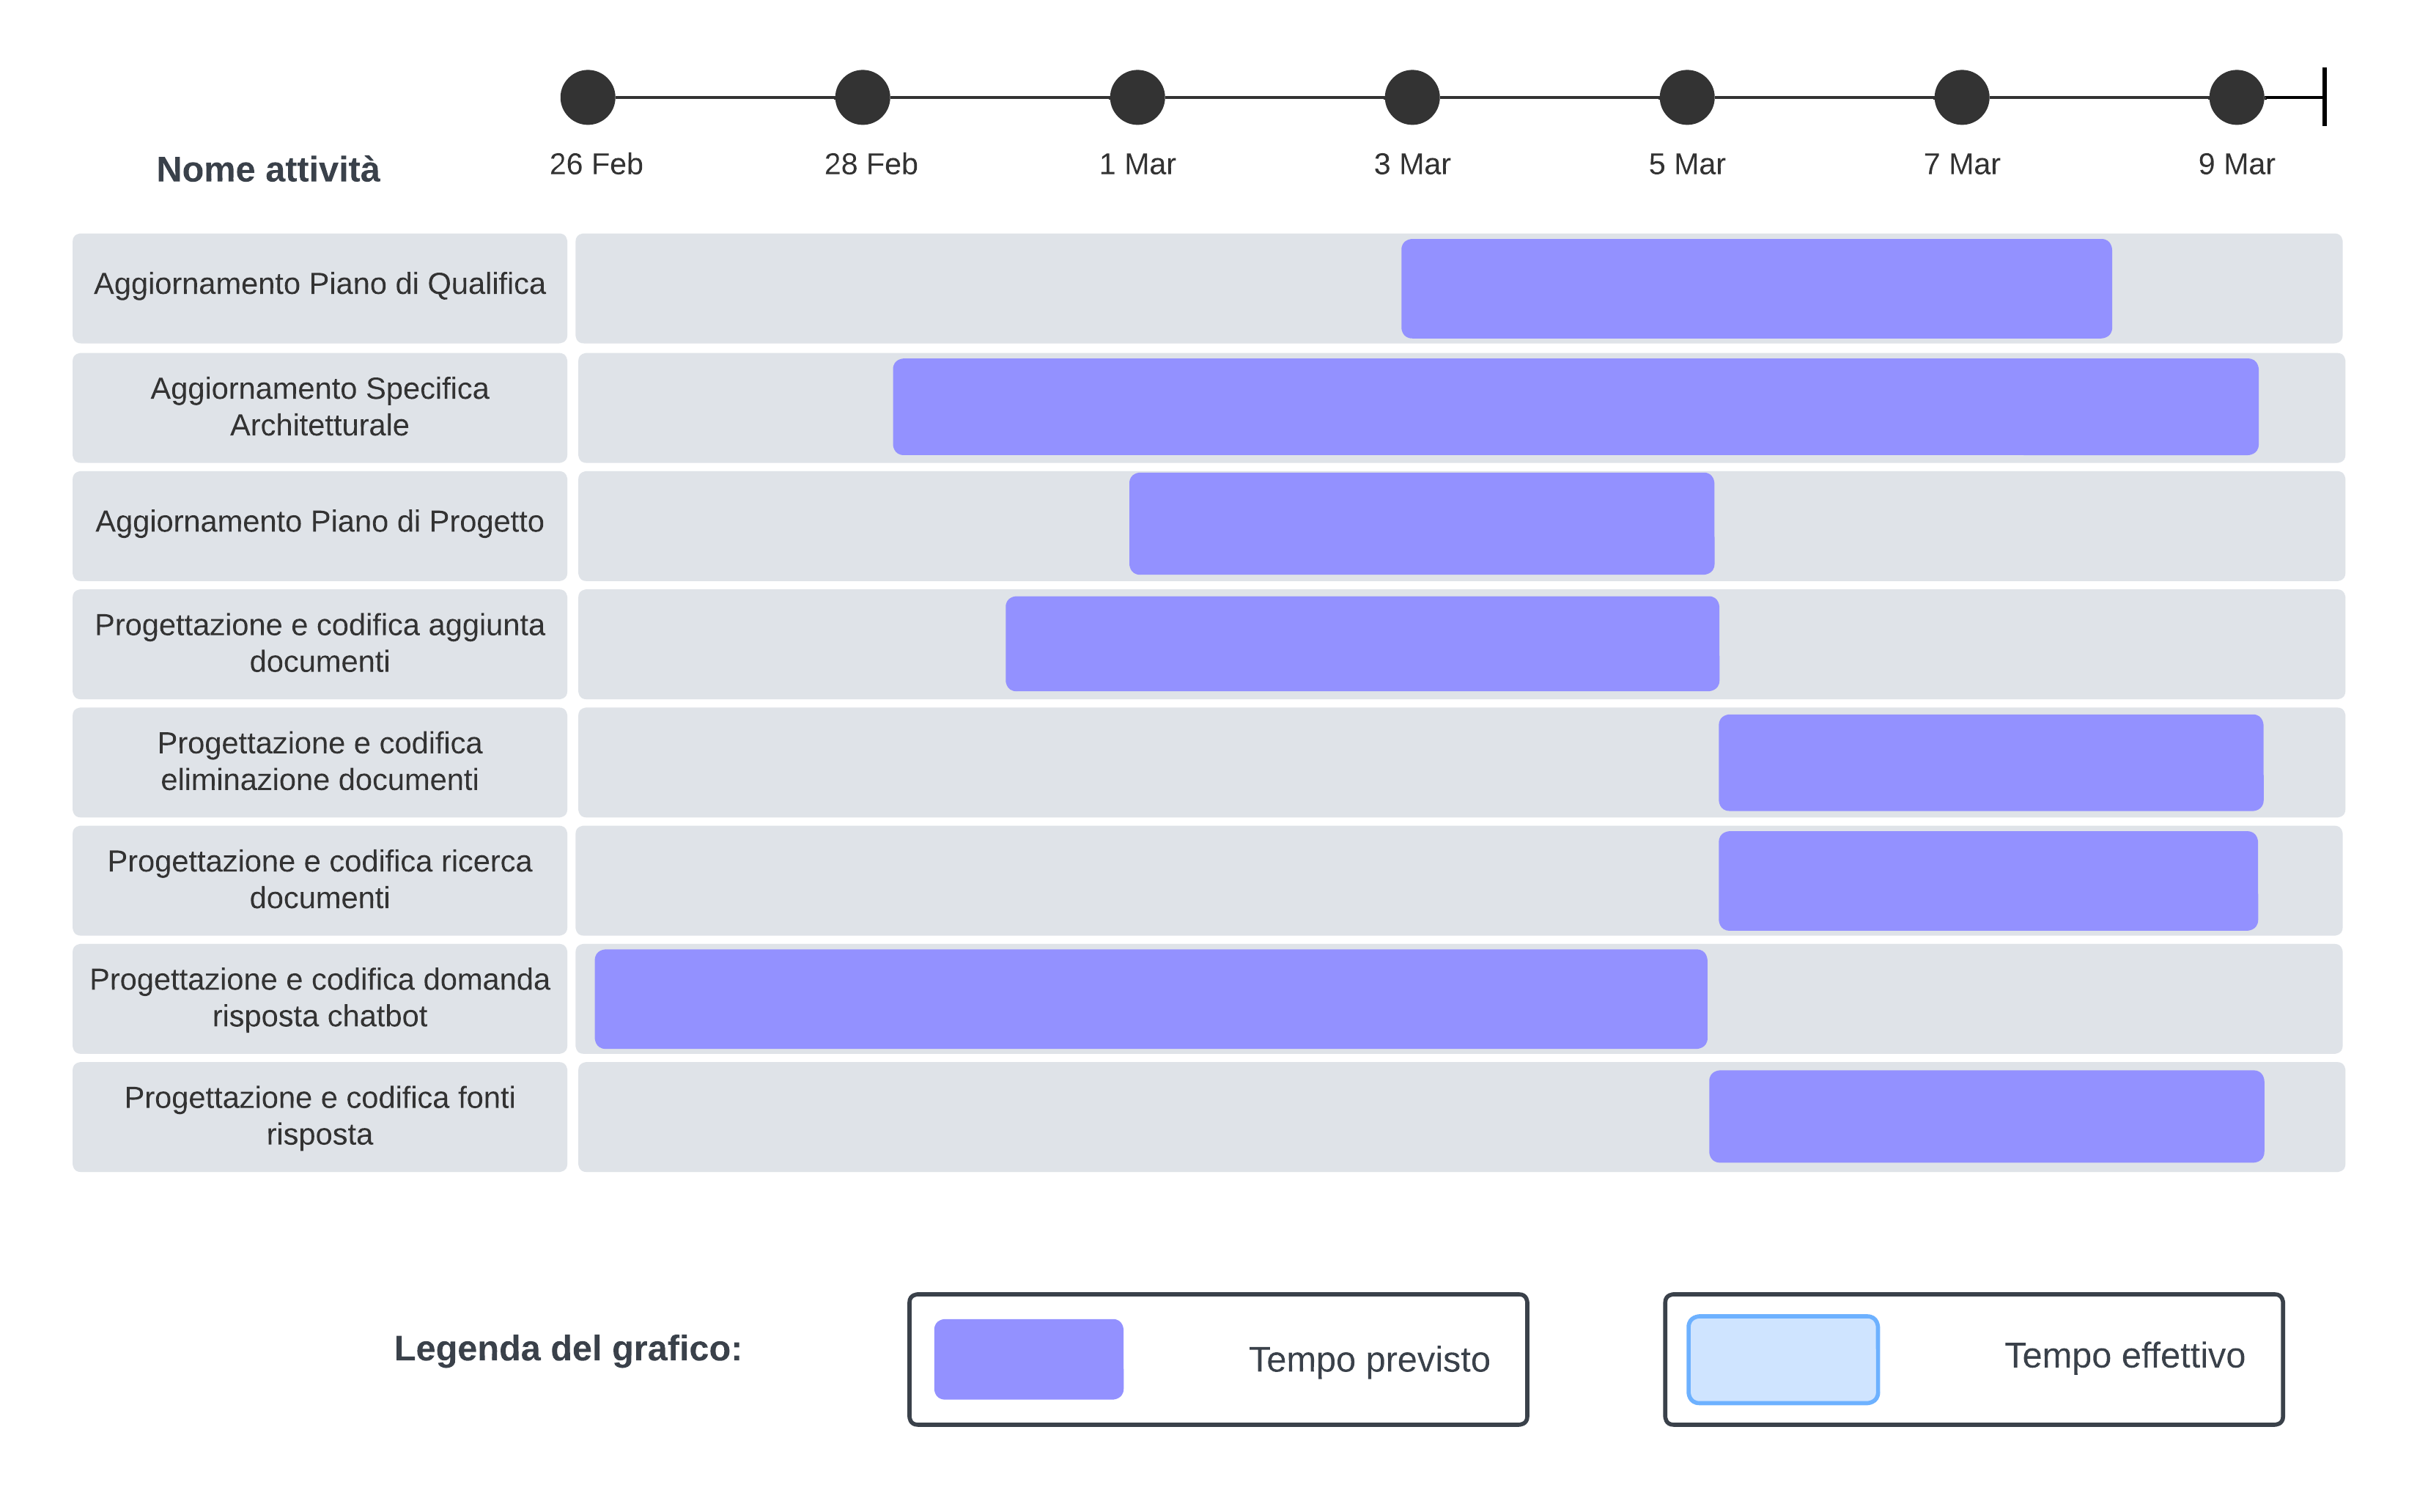
\includegraphics[width=\textwidth]{Roadmap9sprint.png}
    \caption{Diagramma di Gantt del nono sprint}
    \label{fig:roadmaps9s} 
\end{figure}

\subsection{Decimo sprint: 2024/03/11 - 2024/03/24}
\section{Obiettivi}
\begin{itemize}
    \item Aggiornamento Piano di Qualifica;
    \item Aggiornamento Specifica Architetturale;
    \item Aggiornamento Piano di Progetto;
    \item Progettazione e codifica chat thread
    \item Progettazione e codifica chat history
    \item Progettazuibe e codifica dei tag
\end{itemize}

\begin{figure}[h!]
    \centering
    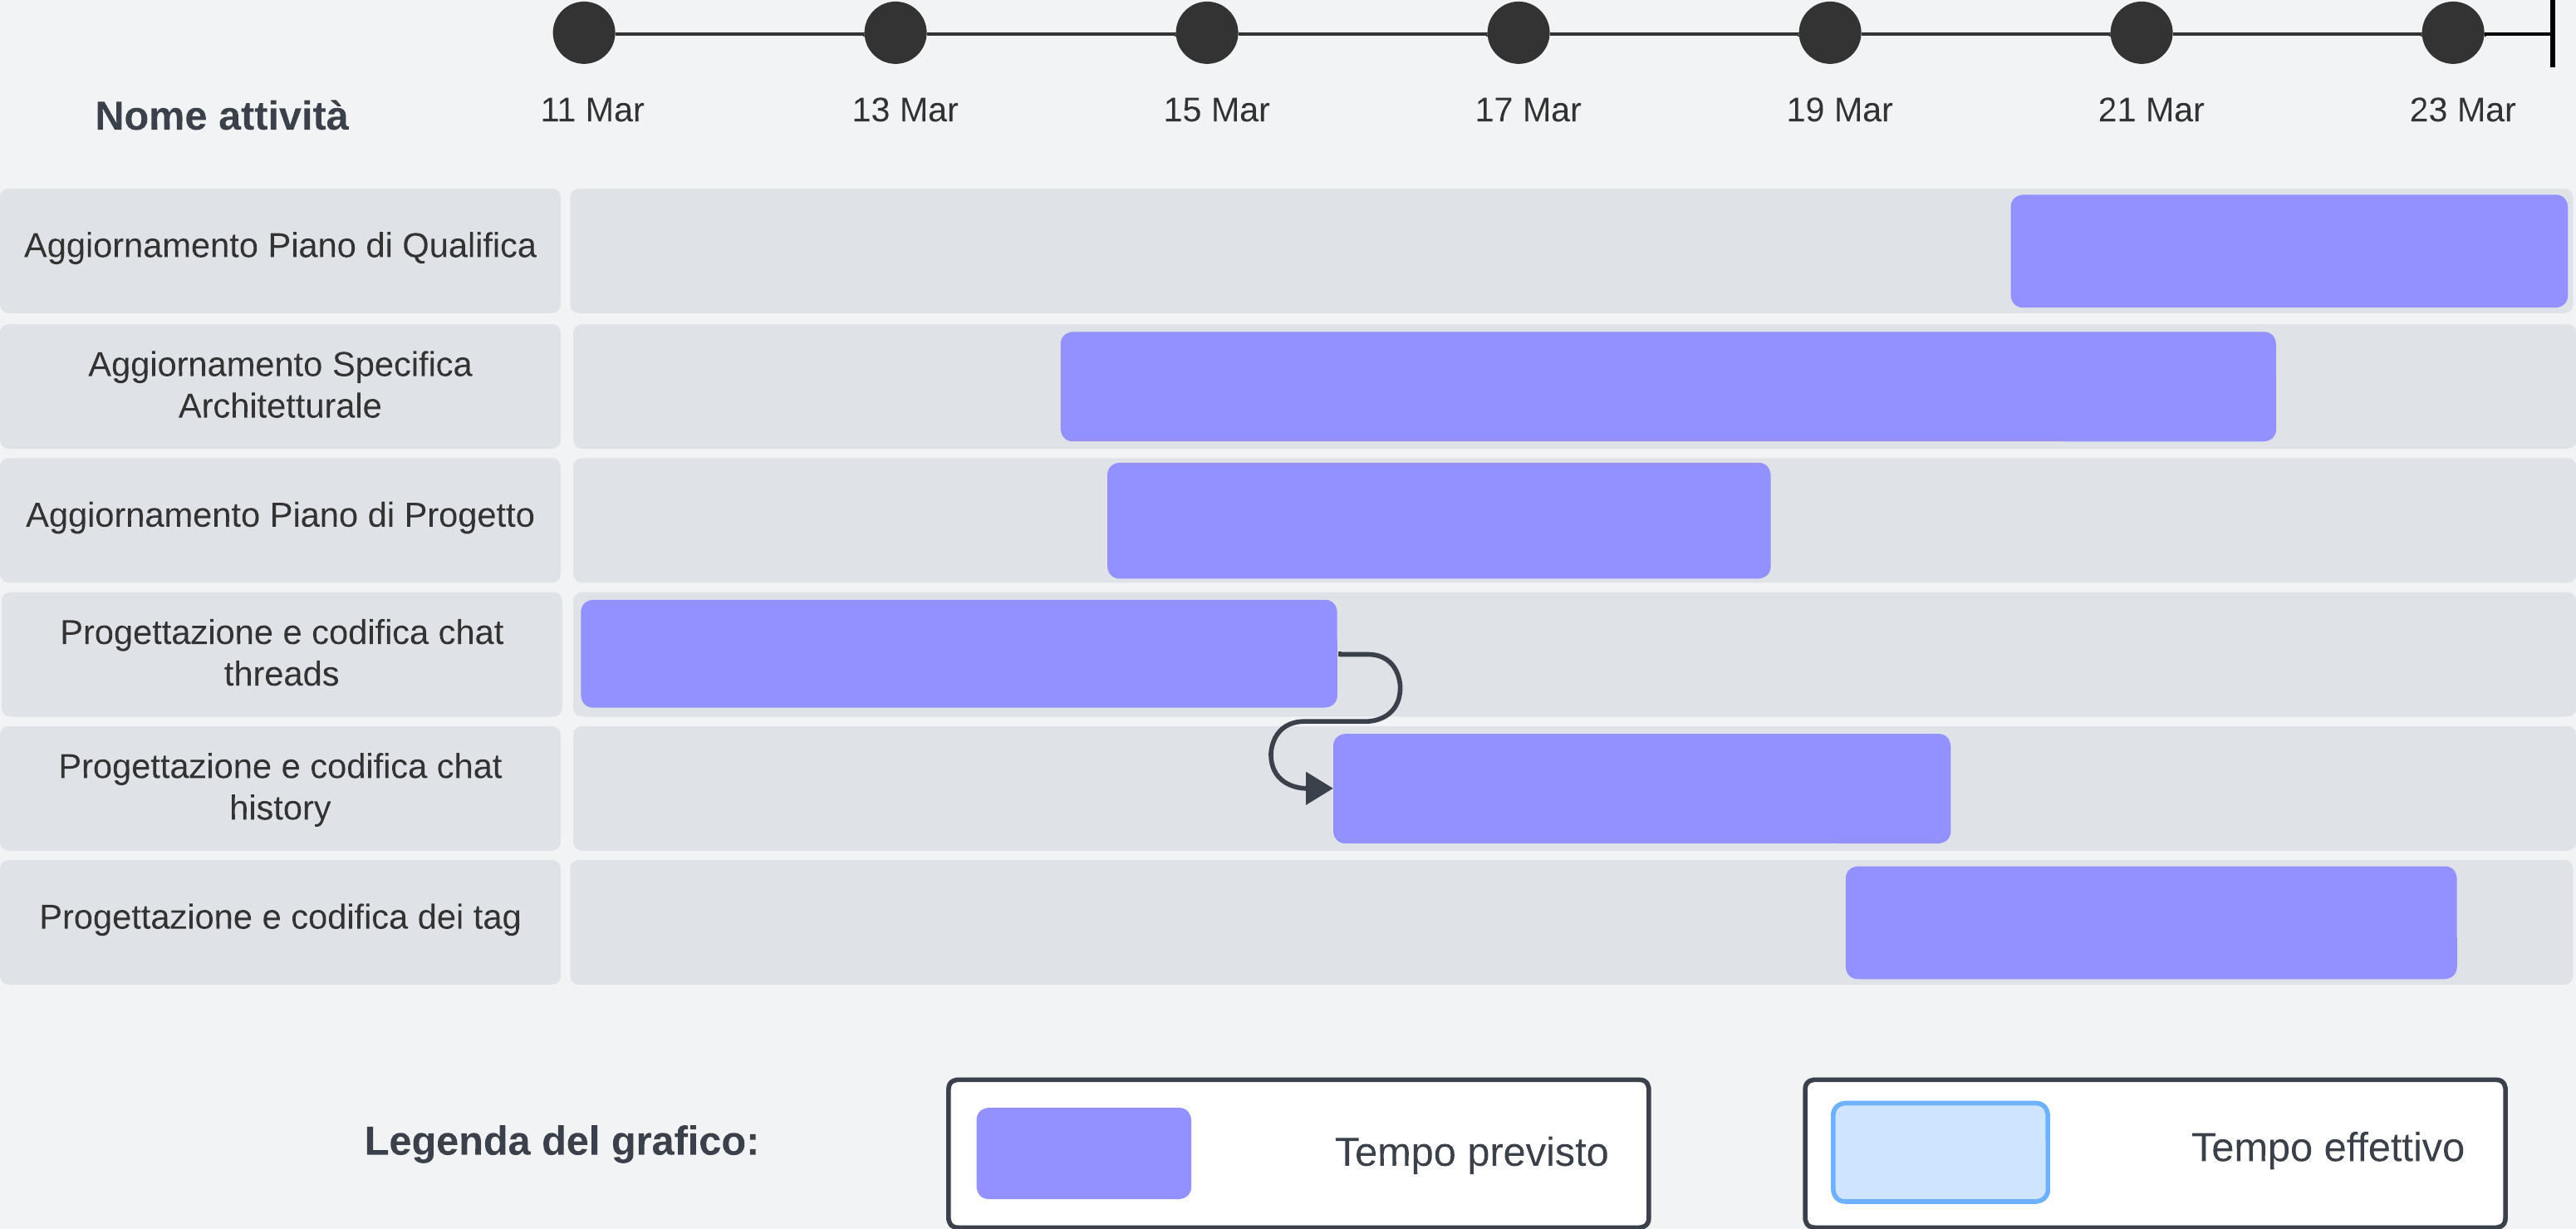
\includegraphics[width=\textwidth]{Roadmap10sprint.png} %aggiornare al prossimo sprint
    \caption{Diagramma di Gantt del decimo sprint}
    \label{fig:roadmaps10s}
\end{figure}
\newpage
